\documentclass[a4paper]{report}
\pagestyle{headings}
\usepackage{hyperref}
\usepackage{listings}
\usepackage{graphicx}
\usepackage{hyperref}
\usepackage{color}
\lstset{language=bash}
\lstset{numbers=right}
\lstset{breaklines}
\title{Lab Report for Object-oriented Programming course \newline
 Lab 3: Linkage}
\author{Wang, Chen \\ 16307110064 \\ School of Software\\ Fudan University}
\date{\today}
\bibliographystyle{plain}
\begin{document}
\maketitle

\tableofcontents

\chapter{Understanding Internal and External Linkage}
\section{Requirements}
In this part, we are going to analyze the running result of the following short program and will try to make some subtle modifications whose change will result in the complete change of the result.
The codes are shown below.

\subsection{header.h}
\begin{lstlisting}[language=C++]
#ifndef LAB3_HEAER_H
#define LAB3_HEAER_H

static int variable = 0;
extern int variable2;
#endif //LAB3_HEAER_H

\end{lstlisting}


\subsection{file1.h}
\begin{lstlisting}[language=C++]
#ifndef LAB3_FILE1_H
#define LAB3_FILE1_H
void function1();

#endif //LAB3_FILE1_H

\end{lstlisting}

\subsection{file2.h}
\begin{lstlisting}[language=C++]
#ifndef LAB3_FILE2_H
#define LAB3_FILE2_H
void function2();

#endif //LAB3_FILE2_H

\end{lstlisting}


\subsection{file1.cpp}
\begin{lstlisting}[language=C++]
#include "header.h"

void function1() {
    variable = 1;
    variable2 = 1;
}
\end{lstlisting}

\subsection{file2.cpp}
\begin{lstlisting}[language=C++]
#include "header.h"
void function2() {
    variable = 2;
    variable2 = 2;

}
\end{lstlisting}

\subsection{main.cpp}
\begin{lstlisting}[language=C++]
#include <iostream>
#include "header.h"
#include "file1.h"
#include "file2.h"
int variable2;

int main() {
    function1();
    function2();

    std::cout << variable << std::endl;
    std::cout << variable2 << std::endl;
    return 0;
}
\end{lstlisting}



\section{Execution result}
The result of the execution is shown in the Figure \ref{1} below.

\begin{figure}
  \centering
  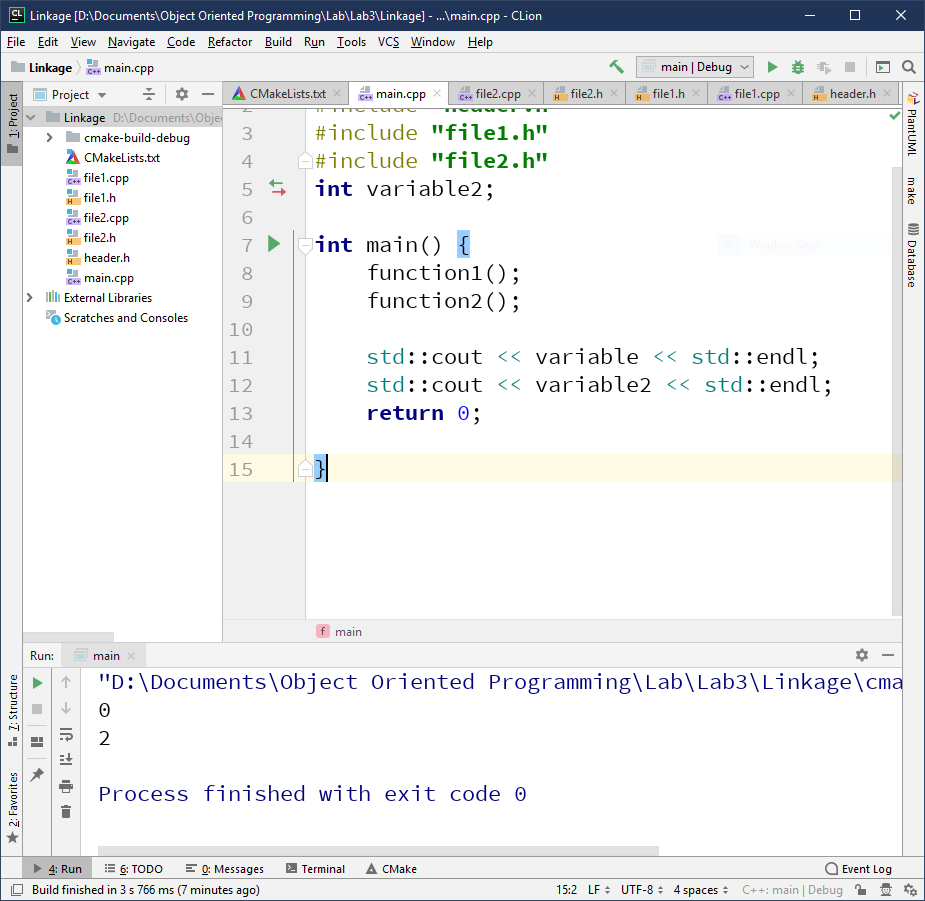
\includegraphics[scale=0.5]{result1.PNG}
  \caption{Execute Results}\label{1}
\end{figure}
\section{Analysis for the result of static variable}
From the C++ language standards, we can know that the \emph{static} keyword has different implications and effects in two different occasions. In this project, the keyword appears before the definition of the global variable outside from any methods. In this case, the \emph{static} keyword has the effect that the variable is only accessible in the specified file, i.e. having a \emph{file scope}.
\par
More specifically, in this project there are three \textbf{cpp} files in this project, each of them including the \emph{header.h} header file where a static variable is declared. In this case, each of the three files has a version of the static variable \emph{variable}. Therefore, the methods \emph{function1} and \emph{function2} will have no effect to the variable \emph{variable} in the \emph{main} method. Hence, the printing result is unchanged.

\section{Analysis for the result of global variable}
As to another part of this lab, the printing result of \emph{variable2}, is a typical example of a global variable. Nevertheless, one slightly point making the analysis more complex is that the \emph{external} keyword is used to make the global variable declared and defined at different places. 
\par
More specifically, in this project, the variable \emph{variable2} is declared in \emph{header.h} with an \emph{external} keyword, indicating that this variable will be defined somewhere else in this project. Then in the file \emph{main.cpp} this variable is defined. Therefore, this is a typical example of global variable and all the functions are modifying the same version of the variable. Therefore, the \emph{main} function will print the result after being changed in the other functions.

\section{Task 1.2: External declaration with definition at the same place}
The result of the change is shown in the Figure \ref{2} below, indicating an compiling error.


\begin{figure}
  \centering
  \includegraphics[scale=0.5]{Onetow.PNG}
  \caption{Execute Results of Task 1.2}\label{2}
\end{figure}


As per have stated above, an \emph{extern} keyword indicates that this variable is defined somewhere else in this file, hence it cannot be used the same time as definition. Therefore, such change will lead to a compiling error.
\section{Task 1.3: External declaration without definition}

The result of the change is shown in the Figure \ref{3} below, indicating an compiling error.


\begin{figure}
  \centering
  \includegraphics[scale=0.5]{Onethree.PNG}
  \caption{Execute Results of Task 1.3}\label{3}
\end{figure}


As per have stated above, an \emph{extern} keyword indicates that this variable is defined somewhere else in this file, hence it will cause a compiling error if no definition is made through out the project file.


\chapter{Understanding Name Space}
\section{Task 2.2 Duplicate variable naming in separate name spaces}
In this task, we are going to use the name space mechanism, create two variables with the same name but different values and print them.
\par
Here in my implementation, I declared two name spaces called \textbf{a} and \textbf{b} separately and then a variable named \textbf{a} in each name space but different value. Then in the \emph{main} method, these two variables are printed separately, we can see the result that they have different values printed. The result is shown in the Figure \ref{4} below.


\begin{figure}
  \centering
  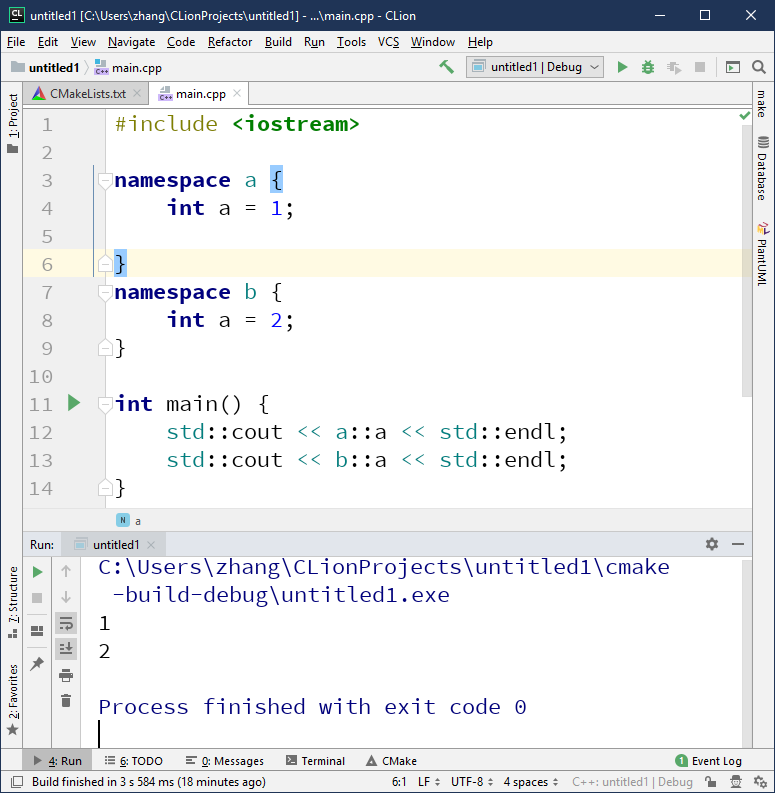
\includegraphics[scale=0.5]{TwoOne.PNG}
  \caption{Execute Results of Task 2.1}\label{4}
\end{figure}

\section{Task 2.2 Extended namespace}
In this task, I will need to duplicately declare the namespace of the same name in two files. The space of the first file defines ``ab=1; cd=2'', and the space of the second file is defined, ``ab=3;bc=4'' Finally, print the value in the namespace in the main function.
\par
Here in my implementation, I declared a name space called \textbf{a} in two separate files and then assigned different values to the variables as stated. Then in the \emph{main} method, these three variables are printed separately, we can see the result that this project cannot be compiled due to duplicate variable definition in the same name space. The result is shown in the Figure \ref{5} below.

\begin{figure}
  \centering
  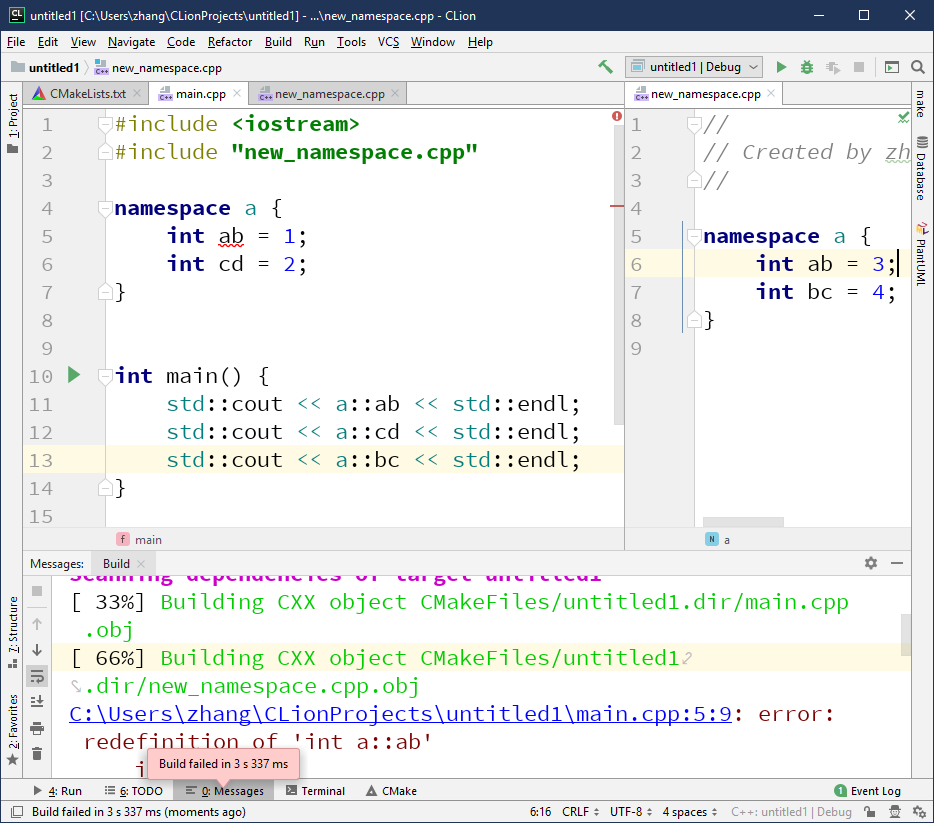
\includegraphics[scale=0.5]{TwoTwo.PNG}
  \caption{Execute Results of Task 2.2}\label{5}
\end{figure}

\chapter{Compare with Typescript Name Space}

\section{Modules in TypeScript}
\emph{\textbf{A note about terminology}: It’s important to note that in TypeScript 1.5, the nomenclature has changed. ``Internal modules'' are now ``namespaces''. ``External modules'' are now simply ``modules'', as to align with ECMAScript 2015\footnote{Ecma International. (2019, May 5). ECMAScript 2015 Language Specification – ECMA-262 6th Edition. In \emph{Ecma International}. Retrieved 08:23, May 11, 2019, from \url{http://www.ecma-international.org/ecma-262/6.0/}}'s terminology, (namely that \textcolor[rgb]{0.749,0.255,0.29}{module X \{ } is equivalent to the now-preferred \textcolor[rgb]{0.749,0.255,0.29}{namespace X \{} ).}
\subsection{Introduction}
Starting with ECMAScript 2015, JavaScript has a concept of modules. TypeScript shares this concept.
\par
Modules are executed within their own scope, not in the global scope; this means that variables, functions, classes, etc. declared in a module are not visible outside the module unless they are explicitly exported using one of the \textcolor[rgb]{0.749,0.255,0.29}{export} forms. Conversely, to consume a variable, function, class, interface, etc. exported from a different module, it has to be imported using one of the \textcolor[rgb]{0.749,0.255,0.29}{import} forms.
\par
Modules are declarative; the relationships between modules are specified in terms of imports and exports at the file level.
Modules import one another using a module loader. At runtime the module loader is responsible for locating and executing all dependencies of a module before executing it. Well-known modules loaders used in JavaScript are the CommonJS module loader for Node.js and require.js for Web applications.
\par
In TypeScript, just as in ECMAScript 2015, any file containing a top-level \textcolor[rgb]{0.749,0.255,0.29}{\textbf{import}} or \textcolor[rgb]{0.749,0.255,0.29}{\textbf{export}} is considered a module. Conversely, a file without any top-level \textcolor[rgb]{0.749,0.255,0.29}{\textbf{import}} or \textcolor[rgb]{0.749,0.255,0.29}{\textbf{export}} declarations is treated as a script whose contents are available in the global scope (and therefore to modules as well).
\section{Name space in TypeScript}

\section{Difference and relation between modules and name spaces in TypeScript}

\section{Internal Linkage in C++}

\section{External Linkage in C++}

\section{Name space in C++}

\section{Difference and relation between TypeScript module and C++ internal linkage}

\section{Difference and relation between TypeScript module and C++ external linkage}

\section{Difference and relation between TypeScript module and C++ name space}

\section{Difference and relation between TypeScript name space and C++ internal linkage}

\section{Difference and relation between TypeScript name space and C++ external linkage}

\section{Difference and relation between TypeScript name space and C++ name space}

\begin{thebibliography}{A}

\bibitem{1}
Wikipedia contributors. (2019, May 5). TypeScript. In \emph{Wikipedia, The Free Encyclopedia}. Retrieved 08:23, May 11, 2019, from \url{https://en.wikipedia.org/w/index.php?title=TypeScript&oldid=895568490}

\bibitem{2}
Wikipedia contributors. (2019, May 9). JavaScript. In \emph{Wikipedia, The Free Encyclopedia}. Retrieved 08:24, May 11, 2019, from \url{https://en.wikipedia.org/w/index.php?title=JavaScript&oldid=896215789}

\bibitem{3}
Wikipedia contributors. (2019, April 24). C++. In \emph{Wikipedia, The Free Encyclopedia}. Retrieved 08:25, May 11, 2019, from \url{https://en.wikipedia.org/w/index.php?title=C%2B%2B&oldid=893975016}

\bibitem{4}
Wikipedia contributors. (2019, February 27). Object-oriented programming. In \emph{Wikipedia, The Free Encyclopedia}. Retrieved 10:22, March 23, 2019, from \url{https://en.wikipedia.org/w/index.php?title=Object-oriented_programming&oldid=885274966}

\bibitem{5}
Wikipedia contributors. (2019, March 18). Namespace. In \emph{Wikipedia, The Free Encyclopedia}. Retrieved 08:27, May 11, 2019, from \url{https://en.wikipedia.org/w/index.php?title=Namespace&oldid=888324103}
\end{thebibliography}
\end{document} 